%%%%%%%%%%%%%%%%%%%%%%%%%%%%%%%%%%%%%%%%%%%%%%%%%%%%%%%%%%%%%%%%%%%%%%%%%%%%%%%
% RAPPORT ACADEMIQUE AMELIORE - PROJET INFORGANIZER DEVOPS
% Master 1 Intelligence Artificielle / Cloud Computing
% Version amelioree avec analyse critique approfondie
%%%%%%%%%%%%%%%%%%%%%%%%%%%%%%%%%%%%%%%%%%%%%%%%%%%%%%%%%%%%%%%%%%%%%%%%%%%%%%%
\documentclass[12pt,a4paper,french]{report}

% ─── Packages ────────────────────────────────────────────────────────────────
\usepackage[utf8]{inputenc}
\usepackage[T1]{fontenc}
\usepackage[french]{babel}
\usepackage{geometry}
\usepackage{graphicx}
\graphicspath{{./evidence/}}
\usepackage{listings}
\usepackage{xcolor}
\usepackage{hyperref}
\usepackage{fancyhdr}
\usepackage{titlesec}
\usepackage{tocloft}
\usepackage{tabularx}
\usepackage{booktabs}
\usepackage{float}
\usepackage{caption}
\usepackage{subcaption}
\usepackage{enumitem}
\usepackage{amsmath}
\usepackage{longtable}
\usepackage{array}
\usepackage{tikz}
\usepackage{url}
\usetikzlibrary{shapes.geometric, arrows, positioning, fit, backgrounds}

% ─── Geometry ────────────────────────────────────────────────────────────────
\geometry{
    top=2.5cm,
    bottom=2.5cm,
    left=2.5cm,
    right=2.5cm,
    headheight=15pt
}

% ─── Colors ──────────────────────────────────────────────────────────────────
\definecolor{codegreen}{rgb}{0,0.6,0}
\definecolor{codegray}{rgb}{0.5,0.5,0.5}
\definecolor{codepurple}{rgb}{0.58,0,0.82}
\definecolor{backcolour}{rgb}{0.95,0.95,0.92}
\definecolor{awsorange}{RGB}{255,153,0}
\definecolor{dockerblue}{RGB}{0,133,209}
\definecolor{k8sblue}{RGB}{50,108,229}
\definecolor{gitopspurple}{RGB}{102,51,153}

% ─── Listings Style ──────────────────────────────────────────────────────────
\lstdefinestyle{codestyle}{
    backgroundcolor=\color{backcolour},
    commentstyle=\color{codegreen},
    keywordstyle=\color{blue},
    numberstyle=\tiny\color{codegray},
    stringstyle=\color{codepurple},
    basicstyle=\ttfamily\footnotesize,
    breakatwhitespace=false,
    breaklines=true,
    captionpos=b,
    keepspaces=true,
    numbers=left,
    numbersep=5pt,
    showspaces=false,
    showstringspaces=false,
    showtabs=false,
    tabsize=2,
    frame=single
}
\lstset{style=codestyle}

% ─── YAML Language Definition ────────────────────────────────────────────────
\lstdefinelanguage{yaml}{
  keywords={true,false,null,y,n},
  keywordstyle=\color{blue}\bfseries,
  basicstyle=\ttfamily\footnotesize,
  sensitive=false,
  comment=[l]{\#},
  morecomment=[s]{/*}{*/},
  commentstyle=\color{codegreen}\ttfamily,
  stringstyle=\color{codepurple}\ttfamily,
  moredelim=[l][\color{orange}]{-\ },
  morestring=[b]',
  morestring=[b]"
}

% ─── Header/Footer ───────────────────────────────────────────────────────────
\pagestyle{fancy}
\fancyhf{}
\fancyhead[L]{\leftmark}
\fancyhead[R]{InfOrganizer DevOps}
\fancyfoot[C]{\thepage}
\renewcommand{\headrulewidth}{0.4pt}
\renewcommand{\footrulewidth}{0.4pt}

% ─── Hyperref Setup ──────────────────────────────────────────────────────────
\hypersetup{
    colorlinks=true,
    linkcolor=blue,
    filecolor=magenta,
    urlcolor=cyan,
    pdftitle={Rapport DevOps Ameliore - InfOrganizer},
    pdfauthor={Etudiant M1 IA/Cloud}
}

%%%%%%%%%%%%%%%%%%%%%%%%%%%%%%%%%%%%%%%%%%%%%%%%%%%%%%%%%%%%%%%%%%%%%%%%%%%%%%%
% DOCUMENT
%%%%%%%%%%%%%%%%%%%%%%%%%%%%%%%%%%%%%%%%%%%%%%%%%%%%%%%%%%%%%%%%%%%%%%%%%%%%%%%
\begin{document}

%%%%%%%%%%%%%%%%%%%%%%%%%%%%%%%%%%%%%%%%%%%%%%%%%%%%%%%%%%%%%%%%%%%%%%%%%%%%%%%
% PAGE DE GARDE
%%%%%%%%%%%%%%%%%%%%%%%%%%%%%%%%%%%%%%%%%%%%%%%%%%%%%%%%%%%%%%%%%%%%%%%%%%%%%%%
\begin{titlepage}
    \centering
    \vspace*{1cm}

    \textsc{\LARGE Universite Hassan II}\\[0.5cm]
    \textsc{\Large Faculte des Sciences et Techniques}\\[0.3cm]
    \textsc{\large Master 1 - Intelligence Artificielle / Cloud Computing}\\[2cm]

    \rule{\linewidth}{0.5mm}\\[0.4cm]
    {\huge\bfseries Mise en Place d'une Infrastructure DevOps\\[0.2cm]
    avec CI/CD, Kubernetes et GitOps}\\[0.2cm]
    \rule{\linewidth}{0.5mm}\\[1.5cm]

    \textsc{\Large Projet : InfOrganizer}\\[0.3cm]
    \textit{Organisateur d'informations pour candidatures universitaires}\\[2cm]

    \begin{minipage}{0.4\textwidth}
        \begin{flushleft}
            \large
            \textbf{Realise par :}\\
            Ismail Mousdik\\
            Oussama Jounaidi\\
            Anass Erfoudi\\
            Mohamed Eddaudi\\
            
        \end{flushleft}
    \end{minipage}
    ~
    \begin{minipage}{0.4\textwidth}
        \begin{flushright}
            \large
            \textbf{Encadre par :}\\
            Pr. Faouzia Benabbou\\
        \end{flushright}
    \end{minipage}\\[3cm]

    \textsc{\large Annee Universitaire 2025-2026}\\[1cm]

    \vfill

\end{titlepage}

%%%%%%%%%%%%%%%%%%%%%%%%%%%%%%%%%%%%%%%%%%%%%%%%%%%%%%%%%%%%%%%%%%%%%%%%%%%%%%%
% RESUME
%%%%%%%%%%%%%%%%%%%%%%%%%%%%%%%%%%%%%%%%%%%%%%%%%%%%%%%%%%%%%%%%%%%%%%%%%%%%%%%
\chapter*{Resume}
\addcontentsline{toc}{chapter}{Resume}

Ce rapport presente la conception, l'implementation et le deploiement d'une infrastructure DevOps complete pour une application web de gestion de candidatures universitaires. Le projet InfOrganizer illustre l'integration des pratiques modernes du genie logiciel dans un contexte cloud-native.

\textbf{Objectif principal :} Automatiser l'ensemble du cycle de vie applicatif, depuis le developpement jusqu'a la production, en eliminant les interventions manuelles sources d'erreurs et en garantissant la reproductibilite des environnements.

\textbf{Approche methodologique :}
L'architecture repose sur le paradigme GitOps, ou Git constitue la source de verite unique pour l'etat desire du systeme. Cette approche, combinee a l'Infrastructure as Code (IaC), assure une tracabilite complete et une capacite de rollback instantanee.

\textbf{Implementation technique :}
\begin{itemize}[noitemsep]
    \item \textbf{Infrastructure} : AWS (VPC, EC2) provisionnee via Terraform
    \item \textbf{Configuration} : Cluster Kubernetes k3s deploye par Ansible
    \item \textbf{Conteneurisation} : Docker avec build multi-stage et principe du moindre privilege
    \item \textbf{CI/CD} : GitHub Actions avec authentification OIDC (zero credentials statiques)
    \item \textbf{Deploiement} : ArgoCD pour la reconciliation GitOps automatique
\end{itemize}

\textbf{Resultats obtenus :}
Le systeme atteint un temps de deploiement de 1 minute 22 secondes entre le commit et la mise en production, avec zero intervention manuelle. La haute disponibilite est assuree par 2 replicas avec anti-affinite et strategie RollingUpdate.

\textbf{Mots-cles :} DevOps, GitOps, Kubernetes, CI/CD, Terraform, Ansible, Docker, AWS, ArgoCD, OIDC

%%%%%%%%%%%%%%%%%%%%%%%%%%%%%%%%%%%%%%%%%%%%%%%%%%%%%%%%%%%%%%%%%%%%%%%%%%%%%%%
% TABLE DES MATIERES
%%%%%%%%%%%%%%%%%%%%%%%%%%%%%%%%%%%%%%%%%%%%%%%%%%%%%%%%%%%%%%%%%%%%%%%%%%%%%%%
\tableofcontents
\listoffigures
\listoftables
\newpage

%%%%%%%%%%%%%%%%%%%%%%%%%%%%%%%%%%%%%%%%%%%%%%%%%%%%%%%%%%%%%%%%%%%%%%%%%%%%%%%
% CHAPITRE 1 : INTRODUCTION
%%%%%%%%%%%%%%%%%%%%%%%%%%%%%%%%%%%%%%%%%%%%%%%%%%%%%%%%%%%%%%%%%%%%%%%%%%%%%%%
\chapter{Introduction}

\section{Contexte et motivation}

L'industrie du logiciel a connu une transformation profonde avec l'emergence du mouvement DevOps, ne de la necessite de reduire les frictions entre les equipes de developpement et d'operations. Cette evolution repond a plusieurs defis majeurs :

\begin{itemize}
    \item \textbf{Acceleration des cycles de livraison} : Les entreprises doivent deployer des mises a jour plusieurs fois par jour, contre quelques fois par an auparavant.
    \item \textbf{Complexite croissante des infrastructures} : L'adoption du cloud et des microservices multiplie les composants a gerer.
    \item \textbf{Exigences de fiabilite} : Les utilisateurs attendent une disponibilite quasi-permanente des services.
\end{itemize}

Dans ce contexte, ce projet vise a mettre en pratique les concepts DevOps sur un cas d'etude concret : le deploiement d'une application web full-stack dans un environnement cloud.

\section{Problematique}

Le deploiement traditionnel d'applications souffre de plusieurs limitations critiques :

\begin{enumerate}
    \item \textbf{Erreurs humaines} : Les configurations manuelles introduisent des incoherences entre environnements.
    \item \textbf{Dette technique operationnelle} : L'absence de documentation executable rend la reproduction des environnements aleatoire.
    \item \textbf{Temps de deploiement} : Les processus manuels peuvent prendre des heures, voire des jours.
    \item \textbf{Absence de tracabilite} : Il est difficile de savoir qui a modifie quoi et quand.
    \item \textbf{Rollback complexe} : Revenir a une version anterieure necessite souvent une intervention manuelle delicate.
\end{enumerate}

\textbf{Question de recherche :} Comment concevoir une infrastructure permettant un deploiement automatise, reproductible et auditable, tout en maintenant la securite et la haute disponibilite ?

\section{Objectifs}

Ce projet poursuit les objectifs suivants, classes par priorite :

\begin{table}[H]
    \centering
    \begin{tabular}{|c|l|l|}
        \hline
        \textbf{Priorite} & \textbf{Objectif} & \textbf{Critere de succes} \\
        \hline
        1 & Automatisation complete & Zero intervention manuelle \\
        2 & Reproductibilite & Infrastructure recreable en < 30 min \\
        3 & Securite & Pas de credentials statiques \\
        4 & Haute disponibilite & Zero downtime lors des deploiements \\
        5 & Tracabilite & Audit trail complet via Git \\
        \hline
    \end{tabular}
    \caption{Objectifs du projet et criteres de succes}
    \label{table:objectifs}
\end{table}

\section{Perimetre du projet}

\textbf{Inclus dans le perimetre :}
\begin{itemize}
    \item Provisionnement de l'infrastructure cloud (AWS)
    \item Configuration automatisee des serveurs
    \item Deploiement d'un cluster Kubernetes
    \item Pipeline CI/CD complet
    \item Deploiement GitOps de l'application
\end{itemize}

\textbf{Hors perimetre (perspectives d'amelioration) :}
\begin{itemize}
    \item Monitoring avance (Prometheus/Grafana)
    \item Gestion centralisee des secrets (Vault)
    \item Multi-environnements (staging/production)
\end{itemize}

%%%%%%%%%%%%%%%%%%%%%%%%%%%%%%%%%%%%%%%%%%%%%%%%%%%%%%%%%%%%%%%%%%%%%%%%%%%%%%%
% CHAPITRE 2 : ARCHITECTURE DU SYSTEME
%%%%%%%%%%%%%%%%%%%%%%%%%%%%%%%%%%%%%%%%%%%%%%%%%%%%%%%%%%%%%%%%%%%%%%%%%%%%%%%
\chapter{Architecture du Systeme}

\section{Vision architecturale}

L'architecture adoptee suit le paradigme \textbf{GitOps}, defini par Weaveworks en 2017, qui repose sur quatre principes fondamentaux :

\begin{enumerate}
    \item \textbf{Declaratif} : L'etat desire du systeme est decrit, pas les etapes pour y parvenir.
    \item \textbf{Versionne et immuable} : Git stocke l'historique complet des configurations.
    \item \textbf{Tire automatiquement} : Un agent surveille Git et applique les changements.
    \item \textbf{Reconciliation continue} : L'agent corrige toute derive entre l'etat desire et l'etat reel.
\end{enumerate}

Cette approche a ete choisie plutot qu'un modele push traditionnel (ou le CI pousse directement vers le cluster) pour plusieurs raisons :
\begin{itemize}
    \item \textbf{Securite} : Le CI n'a pas besoin d'acces direct au cluster Kubernetes.
    \item \textbf{Auditabilite} : Chaque changement est trace dans Git.
    \item \textbf{Self-healing} : ArgoCD corrige automatiquement les modifications manuelles non autorisees.
\end{itemize}

\section{Vue logique de l'architecture}

\begin{figure}[H]
    \centering
    \begin{tikzpicture}[
        node distance=2.2cm and 4cm,
        box/.style={rectangle, draw, rounded corners, minimum width=2.8cm, minimum height=1cm, align=center, fill=blue!10, font=\footnotesize},
        aws/.style={rectangle, draw, rounded corners, minimum width=2.8cm, minimum height=1cm, align=center, fill=orange!20, font=\footnotesize},
        k8s/.style={rectangle, draw, rounded corners, minimum width=2.8cm, minimum height=1cm, align=center, fill=blue!30, font=\footnotesize},
        arrow/.style={->, thick, >=stealth},
        lbl/.style={font=\scriptsize, fill=white, inner sep=1pt}
    ]
        % Row 1: Developer -> GitHub -> ECR
        \node[box] (dev) {Developpeur};
        \node[box, right=of dev] (github) {GitHub\\Repository};
        \node[aws, right=of github] (ecr) {AWS ECR\\Registry};

        % Row 2: GitHub Actions (below GitHub)
        \node[box, below=of github] (actions) {GitHub\\Actions};

        % Row 3: ArgoCD (below Actions)
        \node[k8s, below=of actions] (argocd) {ArgoCD\\(GitOps)};

        % Row 4: K8s Cluster (below ArgoCD)
        \node[k8s, below=of argocd] (k8s) {Cluster k3s};

        % Row 5: PostgreSQL and App below k8s
        \node[k8s, below left=1.5cm and 1cm of k8s] (postgres) {PostgreSQL\\Database};
        \node[k8s, below right=1.5cm and 1cm of k8s] (app) {InfOrganizer\\(2 replicas)};

        % Arrows - main flow
        \draw[arrow] (dev) -- node[lbl, above] {git push} (github);
        \draw[arrow] (github) -- node[lbl, right] {trigger} (actions);
        \draw[arrow] (actions) -- node[lbl, right] {sync} (argocd);
        \draw[arrow] (argocd) -- node[lbl, right] {deploy} (k8s);

        % K8s to app and postgres
        \draw[arrow] (k8s) -- (app);
        \draw[arrow] (k8s) -- (postgres);

        % App to postgres connection
        \draw[arrow] (app) -- node[lbl, below] {connect} (postgres);

        % GitHub Actions to ECR
        \draw[arrow] (actions.east) -- ++(0.5,0) |- node[lbl, near end, below] {push image} (ecr.south);

        % Update manifest arrow (curved back to GitHub)
        \draw[arrow] (actions.west) -- ++(-0.8,0) |- node[lbl, near start, above] {update manifest} (github.west);

        % ECR to app (pull image)
        \draw[arrow] (ecr.south) -- ++(0,-3) -| node[lbl, near start, right] {pull image} (app.north);

    \end{tikzpicture}
    \caption{Architecture GitOps du systeme}
    \label{fig:architecture}
\end{figure}

\section{Flux de deploiement detaille}

Le deploiement suit un flux en 7 etapes, chacune ayant un role precis :

\begin{enumerate}
    \item \textbf{Commit} : Le developpeur pousse son code sur la branche \texttt{main}.
    \item \textbf{Declenchement CI} : GitHub Actions demarre le workflow \texttt{ci.yml}.
    \item \textbf{Tests} : Job \texttt{test} - execution des tests unitaires avec base PostgreSQL ephemere.
    \item \textbf{Build} : Job \texttt{build-push-ecr} - construction de l'image Docker multi-stage.
    \item \textbf{Publication} : Push de l'image vers AWS ECR avec tag SHA (ex: \texttt{sha-f650335950b4}).
    \item \textbf{Mise a jour GitOps} : Job \texttt{gitops-update} - modification du tag dans \texttt{k8s/deployment.yaml}.
    \item \textbf{Synchronisation} : ArgoCD detecte le changement et applique le nouveau manifest au cluster.
\end{enumerate}

\textbf{Pourquoi ce flux ?}
\begin{itemize}
    \item La separation en 3 jobs permet l'echec rapide : si les tests echouent, on ne gaspille pas de ressources a construire l'image.
    \item Le tag SHA garantit l'immutabilite : chaque commit produit une image unique et tracable.
    \item Le commit \texttt{[skip ci]} evite les boucles infinies de declenchement.
\end{itemize}

\section{Architecture reseau AWS}

L'infrastructure AWS est concue selon le principe de defense en profondeur :

\begin{table}[H]
    \centering
    \begin{tabular}{|l|l|l|}
        \hline
        \textbf{Composant} & \textbf{CIDR/Port} & \textbf{Justification} \\
        \hline
        VPC & 10.0.0.0/16 & Isolation reseau complete \\
        Subnet public & 10.0.1.0/24 & 254 adresses suffisantes \\
        SSH (22) & allowed\_cidr uniquement & Limite a l'IP admin \\
        k3s API (6443) & allowed\_cidr uniquement & Securisation du control plane \\
        NodePort (30080) & 0.0.0.0/0 & Acces public a l'application \\
        Intra-cluster & self & Communication pods libre \\
        \hline
    \end{tabular}
    \caption{Configuration reseau et justifications}
    \label{table:network}
\end{table}

%%%%%%%%%%%%%%%%%%%%%%%%%%%%%%%%%%%%%%%%%%%%%%%%%%%%%%%%%%%%%%%%%%%%%%%%%%%%%%%
% CHAPITRE 3 : TECHNOLOGIES ET OUTILS
%%%%%%%%%%%%%%%%%%%%%%%%%%%%%%%%%%%%%%%%%%%%%%%%%%%%%%%%%%%%%%%%%%%%%%%%%%%%%%%
\chapter{Technologies et Outils}

\section{Choix technologiques et justifications}

Chaque technologie a ete selectionnee selon des criteres precis. Cette section explique non seulement \textit{quoi} mais surtout \textit{pourquoi}.

\subsection{Docker : Conteneurisation}

\textbf{Pourquoi Docker ?}
\begin{itemize}
    \item \textbf{Portabilite} : "Build once, run anywhere" - l'image fonctionne identiquement en dev et en prod.
    \item \textbf{Isolation} : Chaque conteneur a son propre filesystem et reseau.
    \item \textbf{Efficacite} : Partage du kernel avec l'hote, contrairement aux VMs.
\end{itemize}

\textbf{Implementation : Build multi-stage}

Le Dockerfile utilise un build en deux stages pour optimiser l'image finale :

\begin{lstlisting}[language=bash, caption=Dockerfile multi-stage (extrait)]
# Stage 1: Installation des dependances uniquement
FROM node:20-alpine AS deps
WORKDIR /app
RUN npm install -g pnpm
COPY package.json pnpm-lock.yaml pnpm-workspace.yaml ./
RUN pnpm install --prod --frozen-lockfile

# Stage 2: Image finale allegee
FROM node:20-alpine
WORKDIR /app
# Securite : utilisateur non-root
RUN addgroup -S appgroup && adduser -S appuser -G appgroup
COPY --from=deps /app/node_modules ./node_modules
COPY server/ ./server/
COPY client/ ./client/
USER appuser
HEALTHCHECK --interval=30s --timeout=5s \
    CMD wget -qO- http://localhost:3000/api/health || exit 1
CMD ["node", "server/server.js"]
\end{lstlisting}

\textbf{Avantages de cette approche :}
\begin{enumerate}
    \item \textbf{Taille reduite} : L'image finale ne contient pas les outils de build (npm, cache).
    \item \textbf{Securite} : L'utilisateur \texttt{appuser} n'a pas les privileges root.
    \item \textbf{Observabilite} : Le HEALTHCHECK integre permet a Docker et Kubernetes de verifier l'etat.
    \item \textbf{Reproductibilite} : \texttt{--frozen-lockfile} garantit les memes versions de dependances.
\end{enumerate}

\textbf{Resultat mesure :} Image de 49.31 Mo (voir preuve ECR, Figure \ref{fig:ecr}).

\subsection{Kubernetes (k3s) : Orchestration}

\textbf{Pourquoi k3s plutot que kubeadm ou EKS ?}

\begin{table}[H]
    \centering
    \begin{tabular}{|l|c|c|c|}
        \hline
        \textbf{Critere} & \textbf{k3s} & \textbf{kubeadm} & \textbf{EKS} \\
        \hline
        Memoire minimale & 512 Mo & 2 Go & N/A (managed) \\
        Temps d'installation & < 1 min & 15-30 min & 15-20 min \\
        Cout & Gratuit & Gratuit & 0.10\$/h/cluster \\
        Compatibilite K8s & 100\% & 100\% & 100\% \\
        Ideal pour & Edge, dev, small clusters & Production & Large scale \\
        \hline
    \end{tabular}
    \caption{Comparaison des distributions Kubernetes}
    \label{table:k8s-comparison}
\end{table}

k3s a ete choisi car :
\begin{itemize}
    \item Le cluster est de petite taille (2 noeuds).
    \item Les ressources EC2 sont limitees (c7i-flex.large, 2 vCPU, 4 Go RAM).
    \item L'installation scriptable s'integre parfaitement avec Ansible.
\end{itemize}

\subsection{Terraform : Infrastructure as Code}

\textbf{Pourquoi Terraform plutot que CloudFormation ou Pulumi ?}

\begin{itemize}
    \item \textbf{Multi-cloud} : Terraform supporte AWS, GCP, Azure avec la meme syntaxe.
    \item \textbf{Etat declaratif} : Le fichier \texttt{terraform.tfstate} trace l'etat reel.
    \item \textbf{Plan avant apply} : \texttt{terraform plan} montre les changements avant execution.
    \item \textbf{Ecosysteme mature} : Providers officiels maintenus par HashiCorp et les cloud providers.
\end{itemize}

\textbf{Ressources provisionnees :}

\begin{lstlisting}[language=bash, caption=Ressources Terraform (extrait de main.tf)]
resource "aws_vpc" "inforganizer" {
  cidr_block           = "10.0.0.0/16"
  enable_dns_hostnames = true
  tags = { Name = "inforganizer-vpc" }
}

resource "aws_instance" "master" {
  ami           = data.aws_ami.ubuntu.id
  instance_type = "c7i-flex.large"
  key_name      = var.key_name
  root_block_device {
    volume_size = 20
    volume_type = "gp3"
  }
  tags = { Name = "inforganizer-master", Role = "master" }
}
\end{lstlisting}

\textbf{Point technique important :} La generation de l'inventaire Ansible utilise \texttt{null\_resource} avec \texttt{local-exec} plutot que \texttt{local\_file}. Ce choix evite l'erreur "Provider produced inconsistent final plan" qui survient quand les IPs ne sont pas encore connues lors du plan.

\subsection{Ansible : Configuration Management}

\textbf{Pourquoi Ansible plutot que Chef ou Puppet ?}

\begin{itemize}
    \item \textbf{Agentless} : Pas de daemon a installer sur les noeuds cibles.
    \item \textbf{Idempotence native} : Les modules garantissent le meme resultat a chaque execution.
    \item \textbf{YAML lisible} : Les playbooks sont comprehensibles sans formation specifique.
    \item \textbf{Integration SSH} : Utilise l'infrastructure SSH existante.
\end{itemize}

\textbf{Structure du playbook principal :}

Le playbook \texttt{install\_k3s.yml} est organise en 5 plays distincts :

\begin{enumerate}
    \item \textbf{Common setup} (tous les noeuds) : Swap, Docker, paquets systeme.
    \item \textbf{Master k3s} : Installation du serveur, recuperation du token.
    \item \textbf{Worker k3s} : Jointure au cluster avec le token.
    \item \textbf{Stabilisation} : Attente que tous les noeuds soient Ready.
    \item \textbf{Bootstrap GitOps} : Installation ArgoCD, secrets, application.
\end{enumerate}

\subsection{GitHub Actions : CI/CD}

\textbf{Pourquoi GitHub Actions plutot que Jenkins ou GitLab CI ?}

\begin{itemize}
    \item \textbf{Integration native} : Pas de serveur CI a maintenir.
    \item \textbf{OIDC natif} : Authentification AWS sans secrets statiques.
    \item \textbf{Marketplace} : Actions prereates pour Docker, AWS, etc.
    \item \textbf{Gratuit} : 2000 minutes/mois pour les repos publics.
\end{itemize}

\textbf{Securite OIDC - Pourquoi c'est crucial :}

L'authentification traditionnelle AWS necessite des credentials statiques (Access Key + Secret Key) stockes en secrets GitHub. Problemes :
\begin{itemize}
    \item Risque de fuite si le secret est expose.
    \item Rotation manuelle necessaire.
    \item Credentials valides indefiniment.
\end{itemize}

Avec OIDC :
\begin{lstlisting}[language=yaml, caption=Authentification OIDC (extrait de ci.yml)]
permissions:
  id-token: write  # Permet de demander un token OIDC

- name: Configure AWS credentials via OIDC
  uses: aws-actions/configure-aws-credentials@v4
  with:
    role-to-assume: ${{ secrets.AWS_GITHUB_ROLE_ARN }}
    aws-region: eu-west-3
\end{lstlisting}

Le token OIDC :
\begin{itemize}
    \item Est genere a chaque execution (pas de stockage).
    \item Expire apres 1 heure maximum.
    \item Est lie au repository et a la branche (impossible de l'utiliser ailleurs).
\end{itemize}

\subsection{ArgoCD : GitOps}

\textbf{Pourquoi ArgoCD plutot que Flux CD ?}

\begin{itemize}
    \item \textbf{UI Web} : Interface graphique pour visualiser l'etat des applications.
    \item \textbf{Sync policies} : Configuration fine du comportement de synchronisation.
    \item \textbf{RBAC integre} : Gestion des permissions par projet.
    \item \textbf{Multi-cluster} : Peut gerer plusieurs clusters depuis une instance centrale.
\end{itemize}

\textbf{Configuration de l'application :}

\begin{lstlisting}[language=yaml, caption=inforganizer-app.yaml]
apiVersion: argoproj.io/v1alpha1
kind: Application
metadata:
  name: inforganizer
  namespace: argocd
spec:
  project: default
  source:
    repoURL: https://github.com/itsma3il/inforganizer-devopss.git
    targetRevision: main
    path: k8s
  destination:
    server: https://kubernetes.default.svc
    namespace: default
  syncPolicy:
    automated:
      prune: true      # Supprime les ressources orphelines
      selfHeal: true   # Corrige les derives manuelles
\end{lstlisting}

\textbf{Comportement du self-heal :} Si un operateur modifie manuellement un deployment (ex: change le nombre de replicas), ArgoCD detecte la derive et restaure l'etat defini dans Git dans les 3 secondes.

%%%%%%%%%%%%%%%%%%%%%%%%%%%%%%%%%%%%%%%%%%%%%%%%%%%%%%%%%%%%%%%%%%%%%%%%%%%%%%%
% CHAPITRE 4 : DETAILS D'IMPLEMENTATION
%%%%%%%%%%%%%%%%%%%%%%%%%%%%%%%%%%%%%%%%%%%%%%%%%%%%%%%%%%%%%%%%%%%%%%%%%%%%%%%
\chapter{Details d'Implementation}

\section{Application InfOrganizer}

\subsection{Description fonctionnelle}

InfOrganizer est une application web permettant aux etudiants d'organiser leurs candidatures universitaires. Elle offre :

\begin{itemize}
    \item Gestion des universites (CRUD) avec statut (Applied, Pending, Accepted, Rejected)
    \item Stockage de notes personnalisees avec champs dynamiques
    \item Systeme de rappels avec dates
    \item Authentification securisee par JWT
    \item Interface bilingue (francais/anglais)
\end{itemize}

\subsection{Architecture technique}

\begin{table}[H]
    \centering
    \begin{tabular}{|l|l|l|}
        \hline
        \textbf{Composant} & \textbf{Technologie} & \textbf{Role} \\
        \hline
        Backend & Node.js 20 + Express & API REST \\
        Base de donnees & PostgreSQL 16 & Persistance \\
        Authentification & JWT (jsonwebtoken) & Sessions stateless \\
        Hachage mots de passe & bcryptjs (cost 12) & Securite \\
        Frontend & HTML/CSS/JS vanilla & Interface utilisateur \\
        \hline
    \end{tabular}
    \caption{Stack technique de l'application}
    \label{table:stack}
\end{table}

\subsection{Schema de base de donnees}

\begin{lstlisting}[language=SQL, caption=Schema PostgreSQL (simplifie)]
CREATE TABLE users (
    id            SERIAL PRIMARY KEY,
    email         TEXT UNIQUE NOT NULL,
    password_hash TEXT NOT NULL,
    created_at    TEXT NOT NULL
);

CREATE TABLE info_notes (
    id         SERIAL PRIMARY KEY,
    user_id    INTEGER REFERENCES users(id) ON DELETE CASCADE,
    name       TEXT NOT NULL,
    created_at TEXT NOT NULL,
    updated_at TEXT NOT NULL
);

CREATE TABLE universities (
    id         SERIAL PRIMARY KEY,
    note_id    INTEGER REFERENCES info_notes(id) ON DELETE CASCADE,
    name       TEXT NOT NULL,
    type       TEXT DEFAULT 'CI',
    status     TEXT DEFAULT 'Applied'
);

CREATE TABLE reminders (
    id      SERIAL PRIMARY KEY,
    user_id INTEGER REFERENCES users(id) ON DELETE CASCADE,
    text    TEXT NOT NULL,
    date    TEXT NOT NULL
);
\end{lstlisting}

\textbf{Choix de conception :}
\begin{itemize}
    \item \texttt{ON DELETE CASCADE} : Suppression en cascade pour maintenir l'integrite referentielle.
    \item Dates en \texttt{TEXT} (ISO 8601) : Simplicite et compatibilite JavaScript.
    \item Index implicites sur les cles primaires et etrangeres.
\end{itemize}

\section{Deployment Kubernetes}

\subsection{Strategie de deploiement}

Le deployment utilise une strategie \texttt{RollingUpdate} avec des parametres specifiques :

\begin{lstlisting}[language=yaml, caption=Strategie RollingUpdate]
spec:
  replicas: 2
  strategy:
    type: RollingUpdate
    rollingUpdate:
      maxUnavailable: 0  # Toujours au moins 2 pods disponibles
      maxSurge: 1        # Au plus 3 pods pendant la transition
\end{lstlisting}

\textbf{Pourquoi ces valeurs ?}
\begin{itemize}
    \item \texttt{maxUnavailable: 0} : Garantit zero downtime - le nouveau pod doit etre Ready avant de terminer l'ancien.
    \item \texttt{maxSurge: 1} : Limite la consommation de ressources pendant le deploiement.
\end{itemize}

\subsection{Init Container : Attente de PostgreSQL}

\begin{lstlisting}[language=yaml, caption=Init container pour dependance]
initContainers:
  - name: wait-for-postgres
    image: postgres:16-alpine
    command: ["sh", "-c",
      "until pg_isready -h postgres -p 5432; do
         echo 'waiting for postgres...'; sleep 3;
       done"]
\end{lstlisting}

\textbf{Pourquoi un init container ?}
\begin{itemize}
    \item L'application Node.js echoue si PostgreSQL n'est pas disponible au demarrage.
    \item L'init container bloque le demarrage du container principal jusqu'a ce que la DB soit prete.
    \item Utilisation de \texttt{postgres:16-alpine} car elle contient \texttt{pg\_isready} (l'image \texttt{busybox} ne l'a pas).
\end{itemize}

\subsection{Anti-affinite pour haute disponibilite}

\begin{lstlisting}[language=yaml, caption=Pod anti-affinity]
affinity:
  podAntiAffinity:
    preferredDuringSchedulingIgnoredDuringExecution:
      - weight: 100
        podAffinityTerm:
          labelSelector:
            matchExpressions:
              - key: app
                operator: In
                values: [inforganizer]
          topologyKey: kubernetes.io/hostname
\end{lstlisting}

\textbf{Explication :}
\begin{itemize}
    \item \texttt{preferred} (pas \texttt{required}) : Le scheduler essaie de placer les pods sur des noeuds differents, mais ne bloque pas si c'est impossible.
    \item \texttt{weight: 100} : Priorite maximale a cette regle.
    \item \texttt{topologyKey: kubernetes.io/hostname} : Distribution par noeud physique.
\end{itemize}

\textbf{Benefice :} Si un noeud tombe en panne, au moins un replica reste disponible sur l'autre noeud.

\subsection{Probes de sante}

\begin{lstlisting}[language=yaml, caption=Liveness et Readiness probes]
livenessProbe:
  httpGet:
    path: /api/health
    port: 3000
  initialDelaySeconds: 15
  periodSeconds: 30

readinessProbe:
  httpGet:
    path: /api/health
    port: 3000
  initialDelaySeconds: 10
  periodSeconds: 10
\end{lstlisting}

\textbf{Difference entre les deux probes :}
\begin{itemize}
    \item \textbf{Liveness} : "Le pod est-il vivant ?" - Si echec, Kubernetes redemarre le pod.
    \item \textbf{Readiness} : "Le pod est-il pret a recevoir du trafic ?" - Si echec, le pod est retire du Service.
\end{itemize}

\textbf{Pourquoi des valeurs differentes ?}
\begin{itemize}
    \item Readiness demarre plus tot (10s vs 15s) pour detecter rapidement les pods prets.
    \item Liveness est moins frequent (30s vs 10s) pour eviter les faux positifs lors de pics de charge.
\end{itemize}

\subsection{Gestion des secrets}

Les secrets sensibles sont injectes via Kubernetes Secrets :

\begin{lstlisting}[language=yaml, caption=Injection des secrets]
env:
  - name: DATABASE_URL
    valueFrom:
      secretKeyRef:
        name: postgres-secret
        key: DATABASE_URL
  - name: JWT_SECRET
    valueFrom:
      secretKeyRef:
        name: postgres-secret
        key: JWT_SECRET
\end{lstlisting}

\textbf{Workflow de creation des secrets :}
\begin{enumerate}
    \item L'operateur definit \texttt{POSTGRES\_PASSWORD} et \texttt{JWT\_SECRET} en variables d'environnement locales.
    \item Ansible lit ces variables via \texttt{lookup('env', 'POSTGRES\_PASSWORD')}.
    \item Ansible genere le manifest Secret via template Jinja2.
    \item Le Secret est applique au cluster avec \texttt{kubectl apply}.
\end{enumerate}

\textbf{Pourquoi cette approche ?}
\begin{itemize}
    \item Les secrets ne sont jamais commites dans Git.
    \item Chaque environnement peut avoir des secrets differents.
    \item Les secrets sont chiffres au repos dans etcd (si configure).
\end{itemize}

\section{Pipeline CI/CD detaille}

\subsection{Job 1 : Tests}

\begin{lstlisting}[language=yaml, caption=Job de tests avec service PostgreSQL]
test:
  runs-on: ubuntu-latest
  services:
    postgres:
      image: postgres:16-alpine
      env:
        POSTGRES_USER: postgres
        POSTGRES_PASSWORD: postgres
        POSTGRES_DB: inforganizer_test
      ports: ["5432:5432"]
      options: >-
        --health-cmd pg_isready
        --health-interval 10s
        --health-timeout 5s
        --health-retries 5
\end{lstlisting}

\textbf{Point cle :} Le service PostgreSQL est demarre comme conteneur sidecar. Les health options garantissent que la DB est prete avant l'execution des tests.

\subsection{Job 2 : Build et Push ECR}

Ce job contient plusieurs validations de securite :

\begin{lstlisting}[language=bash, caption=Validation des secrets (extrait)]
# Verification que le secret existe et est valide
if ! echo "${{ secrets.AWS_ACCOUNT_ID }}" | grep -qE '^[0-9]{12}$'; then
  echo "::error::AWS_ACCOUNT_ID is not a valid 12-digit account ID."
  exit 1
fi

# Validation du format de l'URI avant push
if ! echo "${IMAGE_URI}" | grep -qE '^[0-9]{12}\.dkr\.ecr\.[a-z0-9-]+\.amazonaws\.com/.+$'; then
  echo "::error::Constructed IMAGE_URI is malformed: '${IMAGE_URI}'"
  exit 1
fi
\end{lstlisting}

\textbf{Pourquoi ces validations ?}
Un secret vide ou malconforme pourrait produire une image avec un tag invalide, qui serait ensuite commite dans le manifest Kubernetes, causant un echec de deploiement en cascade.

\subsection{Job 3 : Mise a jour GitOps}

\begin{lstlisting}[language=bash, caption=Mise a jour du manifest avec verification]
# 1. Substitution dans le fichier
sed -i "s|image: ${IMAGE_URI}:.*|image: ${FULL_IMAGE}|" k8s/deployment.yaml

# 2. Verification que la substitution a fonctionne
if ! grep -qF "image: ${FULL_IMAGE}" k8s/deployment.yaml; then
  echo "::error::Verification failed - image not found in deployment.yaml"
  exit 1
fi

# 3. Commit avec [skip ci] pour eviter la boucle infinie
git commit -m "chore(gitops): update image tag to ${IMAGE_TAG} [skip ci]"
\end{lstlisting}

%%%%%%%%%%%%%%%%%%%%%%%%%%%%%%%%%%%%%%%%%%%%%%%%%%%%%%%%%%%%%%%%%%%%%%%%%%%%%%%
% CHAPITRE 5 : PROCESSUS DE DEPLOIEMENT
%%%%%%%%%%%%%%%%%%%%%%%%%%%%%%%%%%%%%%%%%%%%%%%%%%%%%%%%%%%%%%%%%%%%%%%%%%%%%%%
\chapter{Processus de Deploiement}

\section{Procedure de deploiement initial}

\subsection{Phase 1 : Provisionnement AWS (Terraform)}

\begin{lstlisting}[language=bash, caption=Commandes Terraform]
# 1. Configuration
cd terraform
cp terraform.tfvars.example terraform.tfvars
# Editer terraform.tfvars : key_name, allowed_cidr, aws_region

# 2. Initialisation et validation
terraform init
terraform fmt -check
terraform validate

# 3. Planification (verification avant execution)
terraform plan -out=tfplan

# 4. Application
terraform apply tfplan
\end{lstlisting}

\textbf{Duree estimee :} 3-5 minutes (creation EC2, VPC, etc.)

\textbf{Outputs generes :}
\begin{itemize}
    \item \texttt{master\_public\_ip} : IP du noeud control plane
    \item \texttt{worker\_public\_ip} : IP du noeud worker
    \item \texttt{app\_url} : URL d'acces a l'application
    \item \texttt{ansible/inventory.ini} : Inventaire genere automatiquement
\end{itemize}

\subsection{Phase 2 : Configuration du cluster (Ansible)}

\begin{lstlisting}[language=bash, caption=Execution Ansible]
# 1. Definition des secrets (ne jamais commiter ces valeurs)
export POSTGRES_PASSWORD="$(openssl rand -base64 32)"
export JWT_SECRET="$(openssl rand -base64 32)"
export AWS_ACCOUNT_ID="883999922093"

# 2. Execution du playbook
cd ansible
ansible-playbook -i inventory.ini install_k3s.yml

# Duree estimee : 10-15 minutes
\end{lstlisting}

\textbf{Etapes executees par Ansible :}
\begin{enumerate}
    \item Installation des paquets (curl, git, awscli, docker)
    \item Configuration du swap (2 Go) pour eviter les OOM kills
    \item Installation de k3s sur le master
    \item Jointure du worker au cluster
    \item Installation d'ArgoCD
    \item Creation des secrets Kubernetes
    \item Deploiement de l'application ArgoCD
\end{enumerate}

\subsection{Phase 3 : Verification}

\begin{lstlisting}[language=bash, caption=Commandes de verification]
# Connexion au master
ssh -i ~/.ssh/key.pem ubuntu@<MASTER_IP>

# Verification du cluster
sudo k3s kubectl get nodes
# Attendu : 2 noeuds en status Ready

# Verification des pods
sudo k3s kubectl get pods -n default
# Attendu : 2 pods inforganizer Running, 1 pod postgres Running

# Verification d'ArgoCD
sudo k3s kubectl get application -n argocd
# Attendu : inforganizer Synced Healthy

# Test de l'application
curl http://<MASTER_IP>:30080/api/health
# Attendu : {"status":"ok"}
\end{lstlisting}

\section{Deploiement continu automatise}

Apres la configuration initiale, tout deploiement ulterieur est automatique :

\begin{enumerate}
    \item Le developpeur modifie le code et pousse sur \texttt{main}.
    \item GitHub Actions execute les tests, build l'image, la pousse sur ECR.
    \item Le manifest \texttt{k8s/deployment.yaml} est mis a jour avec le nouveau tag.
    \item ArgoCD detecte le changement (polling toutes les 3 secondes par defaut).
    \item ArgoCD applique le nouveau deployment au cluster.
    \item Kubernetes effectue un RollingUpdate : nouveau pod cree, ancien termine.
\end{enumerate}

\textbf{Temps mesure :} 1 minute 22 secondes du commit a l'application deployee (voir Figure \ref{fig:pipeline}).

%%%%%%%%%%%%%%%%%%%%%%%%%%%%%%%%%%%%%%%%%%%%%%%%%%%%%%%%%%%%%%%%%%%%%%%%%%%%%%%
% CHAPITRE 6 : PREUVES ET VALIDATION
%%%%%%%%%%%%%%%%%%%%%%%%%%%%%%%%%%%%%%%%%%%%%%%%%%%%%%%%%%%%%%%%%%%%%%%%%%%%%%%
\chapter{Preuves et Validation}

Cette section presente les preuves d'execution collectees lors du deploiement reel du systeme.

\section{Infrastructure AWS}

\subsection{Instances EC2}

Deux instances EC2 de type \texttt{c7i-flex.large} ont ete provisionnees :
\begin{itemize}
    \item \texttt{inforganizer-master} : Noeud control plane k3s
    \item \texttt{inforganizer-worker} : Noeud worker pour les workloads
\end{itemize}

\begin{figure}[H]
    \centering
    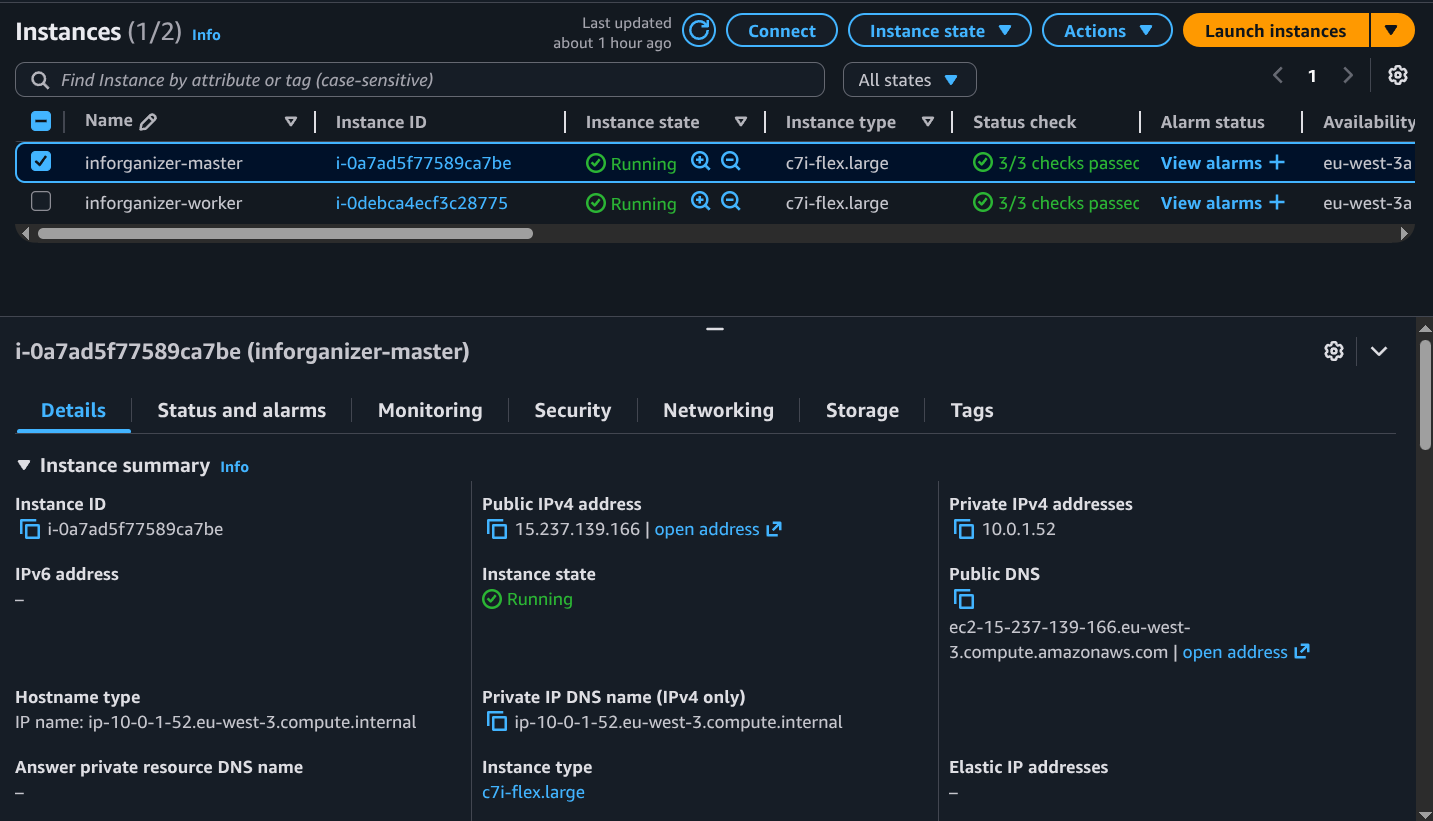
\includegraphics[width=\textwidth]{CAP_01_aws_ec2_instances.png}
    \caption{Instances EC2 provisionnees sur AWS}
    \label{fig:ec2}
\end{figure}

\subsection{Security Groups}

Les groupes de securite ont ete configures pour restreindre l'acces :

\begin{figure}[H]
    \centering
    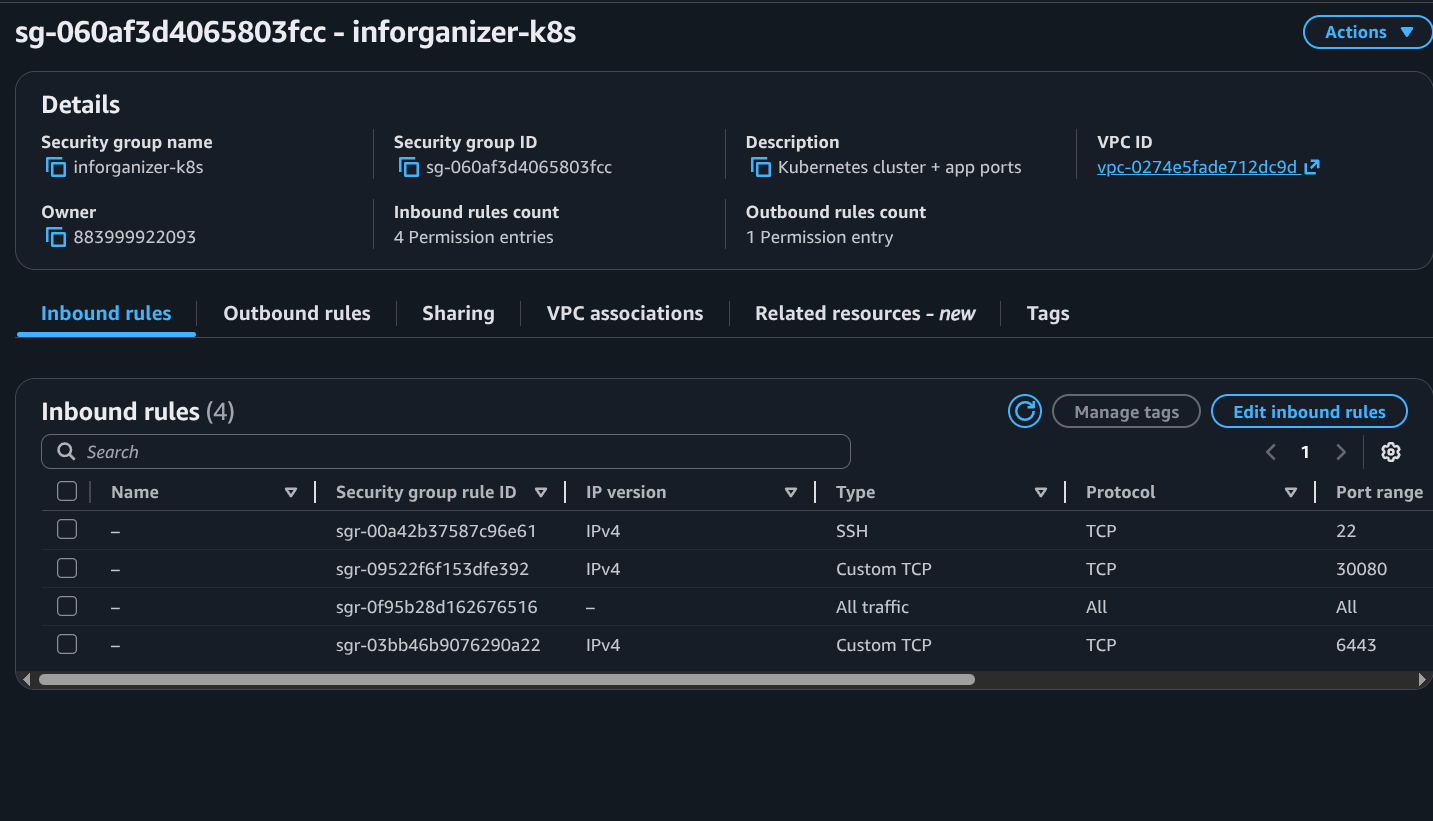
\includegraphics[width=\textwidth]{CAP_02_aws_security_groups.png}
    \caption{Configuration des Security Groups AWS}
    \label{fig:securitygroups}
\end{figure}

\subsection{Configuration IAM OIDC}

Le role \texttt{AWS\_GITHUB\_ROLE\_ARN} a ete configure avec :
\begin{itemize}
    \item Trust relationship : GitHub OIDC provider
    \item Permissions : AmazonEC2ContainerRegistryPowerUser (lecture/ecriture ECR)
    \item Session duration : 1 heure maximum
\end{itemize}

\begin{figure}[H]
    \centering
    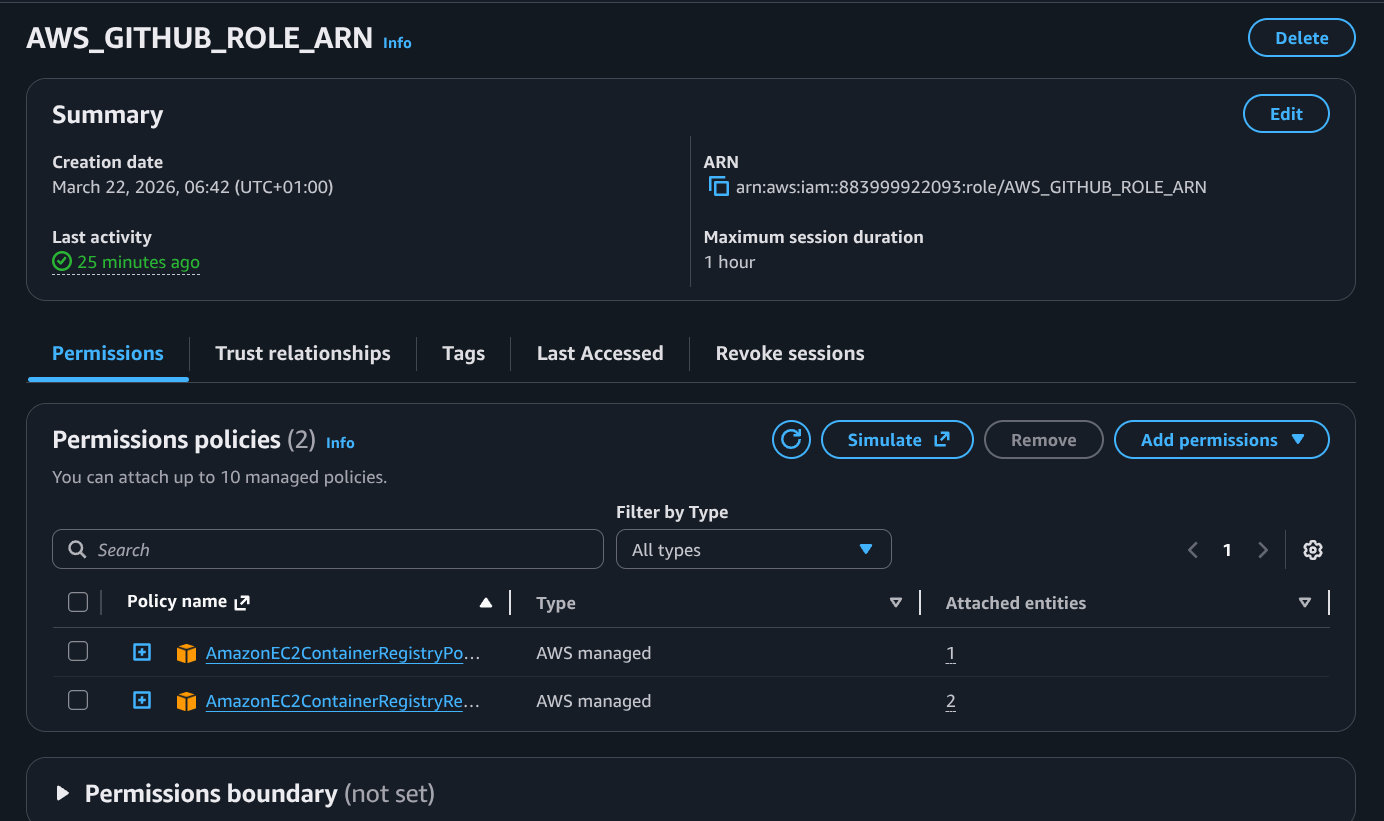
\includegraphics[width=\textwidth]{CAP_03_aws_iam_oidc_role.png}
    \caption{Configuration du role IAM OIDC pour GitHub Actions}
    \label{fig:oidc}
\end{figure}

\section{Provisionnement et Configuration}

\subsection{Terraform Apply}

L'infrastructure a ete provisionnee avec succes via Terraform :

\begin{figure}[H]
    \centering
    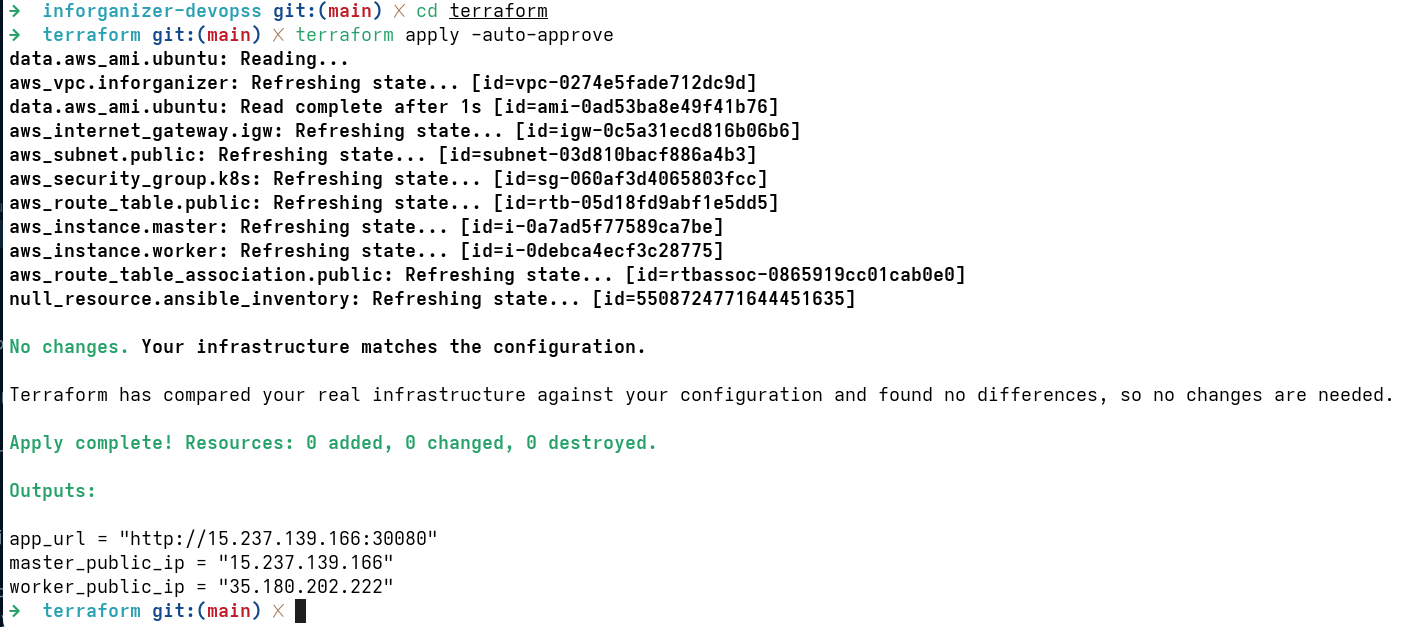
\includegraphics[width=\textwidth]{CAP_04_terraform_apply_success.png}
    \caption{Execution reussie de Terraform apply}
    \label{fig:terraform}
\end{figure}

\subsection{Ansible Playbook}

Le playbook Ansible a configure le cluster k3s avec succes :

\begin{figure}[H]
    \centering
    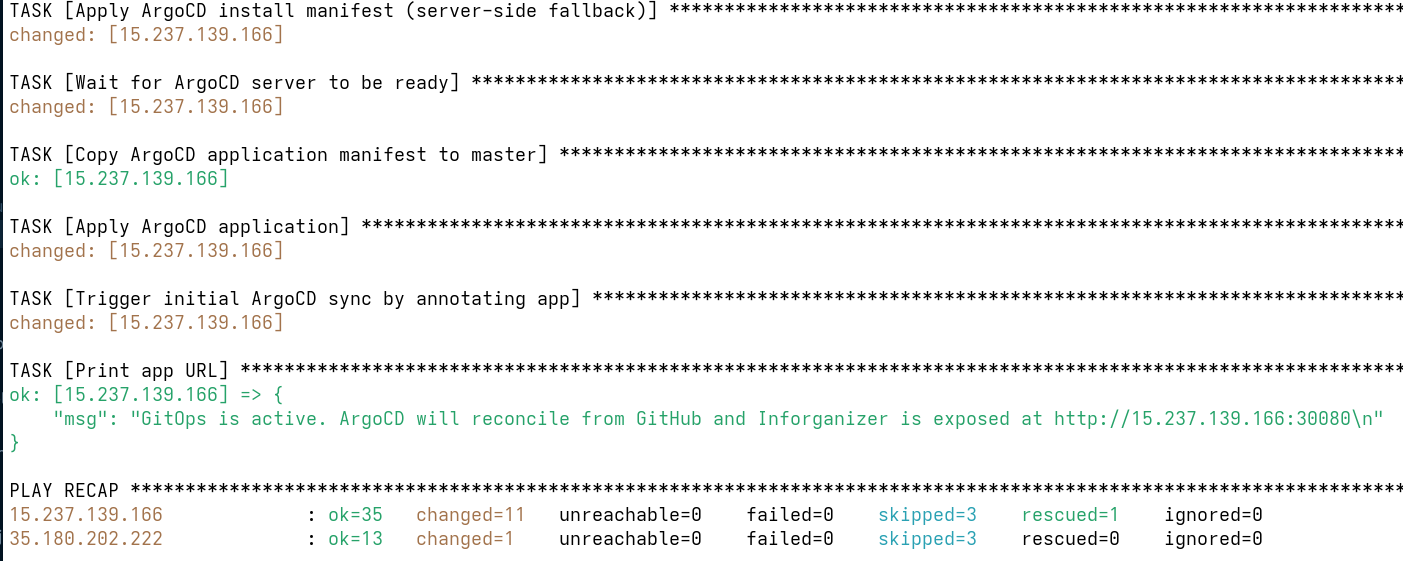
\includegraphics[width=\textwidth]{CAP_05_ansible_play_recap.png}
    \caption{Recap de l'execution du playbook Ansible}
    \label{fig:ansible}
\end{figure}

\section{Cluster Kubernetes}

\subsection{Etat des noeuds}

\begin{figure}[H]
    \centering
    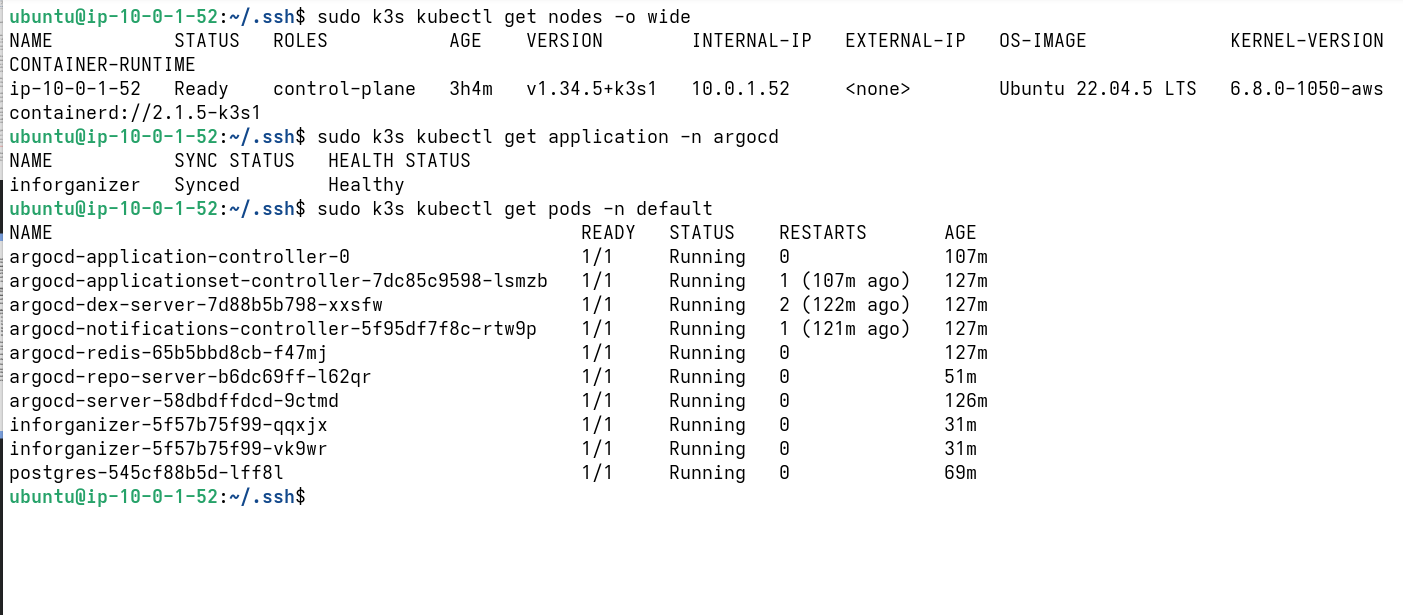
\includegraphics[width=\textwidth]{CAP_06_kubectl_get_nodes.png}
    \caption{Noeuds Kubernetes en etat Ready}
    \label{fig:nodes}
\end{figure}

\subsection{Pods applicatifs}

Deux replicas de l'application sont en execution :
\begin{itemize}
    \item \texttt{inforganizer-5f57b75f99-qqxjx} : Running, Ready 1/1
    \item \texttt{inforganizer-5f57b75f99-vk9wr} : Running, Ready 1/1
\end{itemize}

\begin{figure}[H]
    \centering
    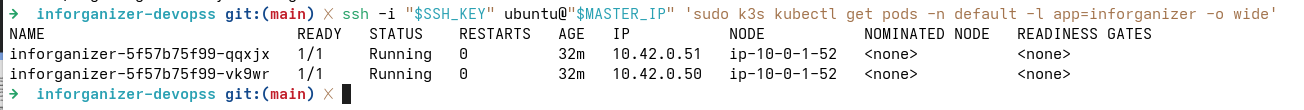
\includegraphics[width=\textwidth]{CAP_07_kubectl_get_pods_app.png}
    \caption{Pods applicatifs en execution}
    \label{fig:pods}
\end{figure}

\subsection{Services exposes}

Le service \texttt{inforganizer} est accessible sur le port 30080 depuis l'exterieur.
Le service \texttt{postgres} reste interne au cluster (ClusterIP).

\begin{figure}[H]
    \centering
    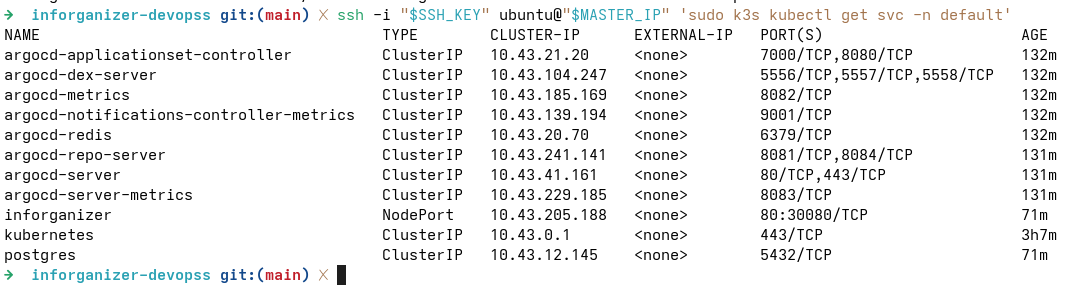
\includegraphics[width=\textwidth]{CAP_08_kubectl_get_svc.png}
    \caption{Services Kubernetes exposes}
    \label{fig:services}
\end{figure}

\subsection{Test de sante de l'API}

L'endpoint de sante de l'application repond correctement :

\begin{figure}[H]
    \centering
    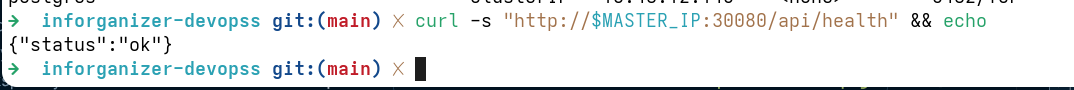
\includegraphics[width=0.8\textwidth]{CAP_09_curl_api_health_ok.png}
    \caption{Test de sante de l'API - reponse OK}
    \label{fig:healthcheck}
\end{figure}

\section{Pipeline CI/CD}

\subsection{Execution reussie}

Le workflow \texttt{CI/CD (GitOps + ECR)} s'est execute avec succes :
\begin{itemize}
    \item \textbf{Commit} : feat(ci): enhance CI/CD pipeline (f650335)
    \item \textbf{Duree totale} : 1 minute 22 secondes
    \item \textbf{Jobs} : Install and Test (35s) + Build and Push (35s) + Update GitOps (5s)
\end{itemize}

\begin{figure}[H]
    \centering
    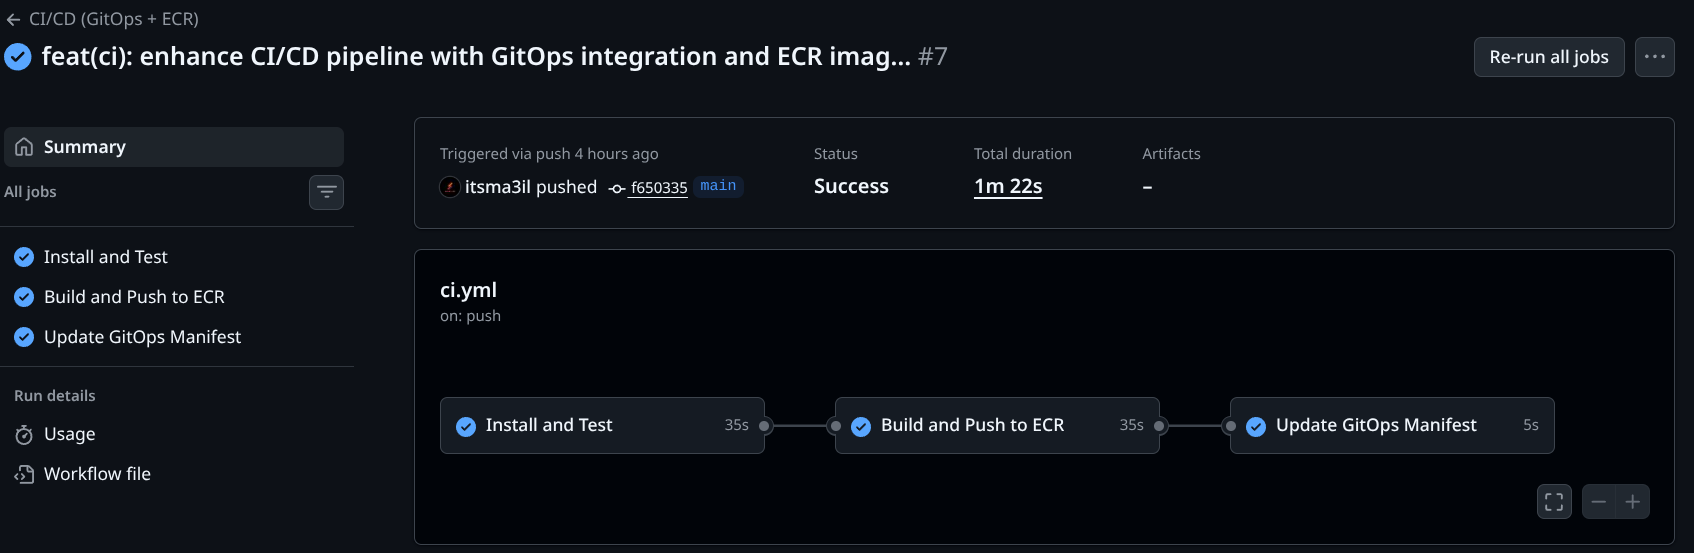
\includegraphics[width=\textwidth]{CAP_10_github_actions_success.png}
    \caption{Pipeline CI/CD execute avec succes}
    \label{fig:pipeline}
\end{figure}

\subsection{Image publiee sur ECR}

L'image a ete publiee avec deux tags :
\begin{itemize}
    \item \texttt{sha-94bbf8f77cb9} : Tag immutable lie au commit
    \item \texttt{latest} : Tag mobile pour faciliter les tests
\end{itemize}

Taille de l'image : 49.31 Mo

\begin{figure}[H]
    \centering
    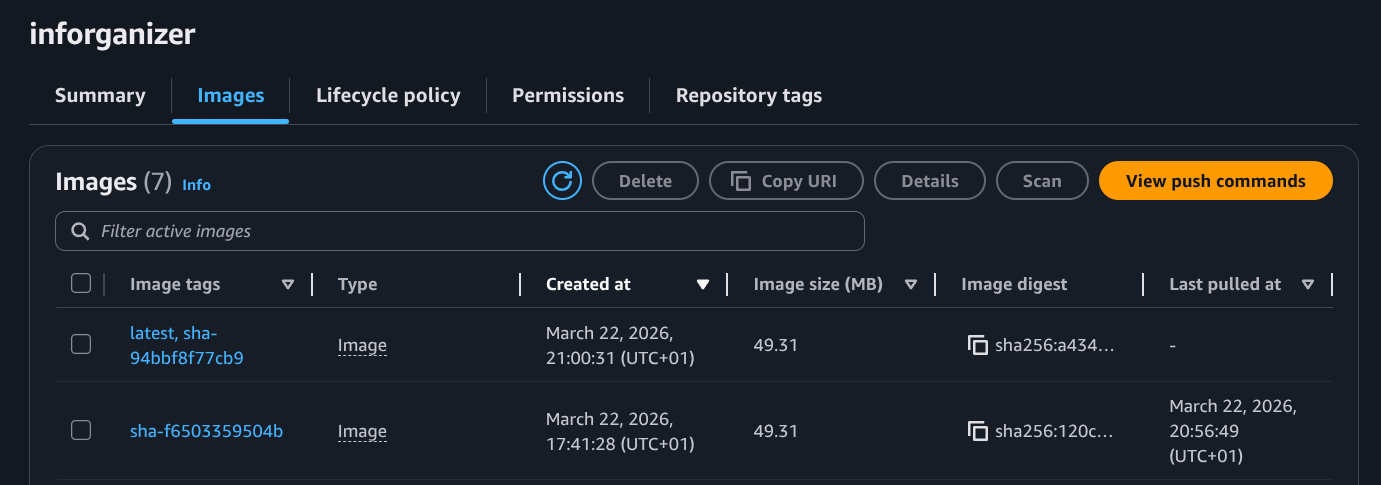
\includegraphics[width=\textwidth]{CAP_11_ecr_image_tag.png}
    \caption{Image Docker publiee sur AWS ECR}
    \label{fig:ecr}
\end{figure}

\section{GitOps ArgoCD}

\subsection{Synchronisation}

L'application \texttt{inforganizer} dans ArgoCD affiche :
\begin{itemize}
    \item \textbf{SYNC STATUS} : Synced (le cluster correspond a Git)
    \item \textbf{HEALTH STATUS} : Healthy (tous les pods sont operationnels)
\end{itemize}

\begin{figure}[H]
    \centering
    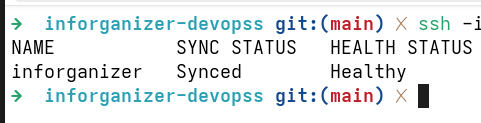
\includegraphics[width=\textwidth]{CAP_12_argocd_synced_healthy.png}
    \caption{ArgoCD - Application synchronisee et saine}
    \label{fig:argocd}
\end{figure}

\section{Tableau recapitulatif des validations}

\begin{table}[H]
    \centering
    \begin{tabular}{|l|l|c|l|}
        \hline
        \textbf{ID} & \textbf{Element valide} & \textbf{Statut} & \textbf{Figure} \\
        \hline
        PREUVE\_01 & Instances EC2 creees & OK & Fig. \ref{fig:ec2} \\
        PREUVE\_02 & Security Groups configures & OK & Fig. \ref{fig:securitygroups} \\
        PREUVE\_03 & IAM OIDC fonctionnel & OK & Fig. \ref{fig:oidc} \\
        PREUVE\_04 & Terraform apply reussi & OK & Fig. \ref{fig:terraform} \\
        PREUVE\_05 & Ansible playbook complet & OK & Fig. \ref{fig:ansible} \\
        PREUVE\_06 & Noeuds k3s Ready & OK & Fig. \ref{fig:nodes} \\
        PREUVE\_07 & Pods Running (2 replicas) & OK & Fig. \ref{fig:pods} \\
        PREUVE\_08 & Service NodePort expose & OK & Fig. \ref{fig:services} \\
        PREUVE\_09 & API Health OK & OK & Fig. \ref{fig:healthcheck} \\
        PREUVE\_10 & Pipeline CI/CD vert & OK & Fig. \ref{fig:pipeline} \\
        PREUVE\_11 & Image publiee sur ECR & OK & Fig. \ref{fig:ecr} \\
        PREUVE\_12 & ArgoCD Synced/Healthy & OK & Fig. \ref{fig:argocd} \\
        \hline
    \end{tabular}
    \caption{Synthese des validations}
    \label{table:validations}
\end{table}

%%%%%%%%%%%%%%%%%%%%%%%%%%%%%%%%%%%%%%%%%%%%%%%%%%%%%%%%%%%%%%%%%%%%%%%%%%%%%%%
% CHAPITRE 7 : DISCUSSION
%%%%%%%%%%%%%%%%%%%%%%%%%%%%%%%%%%%%%%%%%%%%%%%%%%%%%%%%%%%%%%%%%%%%%%%%%%%%%%%
\chapter{Discussion}

\section{Points forts de l'implementation}

\subsection{Automatisation complete}

Le systeme atteint l'objectif de zero intervention manuelle apres la configuration initiale :
\begin{itemize}
    \item Temps de deploiement : 1 min 22s (du commit a la production)
    \item Zero credentials statiques grace a OIDC
    \item Self-healing via ArgoCD
\end{itemize}

\subsection{Securite en profondeur}

Plusieurs couches de securite ont ete implementees :
\begin{enumerate}
    \item \textbf{Infrastructure} : Security Groups restrictifs, SSH limite a une IP.
    \item \textbf{CI/CD} : OIDC elimine le risque de fuite de credentials.
    \item \textbf{Container} : Utilisateur non-root, image minimale Alpine.
    \item \textbf{Kubernetes} : Secrets pour les donnees sensibles, probes de sante.
\end{enumerate}

\subsection{Haute disponibilite}

\begin{itemize}
    \item 2 replicas avec anti-affinite : un noeud peut tomber sans impact utilisateur.
    \item RollingUpdate avec maxUnavailable=0 : zero downtime lors des deploiements.
    \item Base PostgreSQL sur volume persistant : les donnees survivent aux redemarrages.
\end{itemize}

\section{Limites identifiees}

\subsection{Single Point of Failure : Control Plane}

Le cluster utilise un seul noeud master. En cas de panne de ce noeud :
\begin{itemize}
    \item L'API Kubernetes devient inaccessible.
    \item Les pods existants continuent de fonctionner (sur le worker).
    \item Aucun nouveau deploiement ni scaling n'est possible.
\end{itemize}

\textbf{Solution recommandee :} Deployer k3s en mode HA avec 3 noeuds control plane et un load balancer.

\subsection{Absence de monitoring}

Le systeme ne dispose pas de :
\begin{itemize}
    \item Collecte de metriques (CPU, memoire, requetes HTTP).
    \item Alerting en cas d'anomalie.
    \item Dashboard de visualisation.
\end{itemize}

\textbf{Solution recommandee :} Deployer la stack Prometheus + Grafana + AlertManager.

\subsection{Gestion des secrets}

Les secrets sont injectes via variables d'environnement Ansible, ce qui presente des limites :
\begin{itemize}
    \item Pas de rotation automatique.
    \item Pas d'audit trail des acces aux secrets.
    \item Secrets en clair dans la memoire des pods.
\end{itemize}

\textbf{Solution recommandee :} Integrer HashiCorp Vault avec External Secrets Operator.

\subsection{Backup de la base de donnees}

Aucun mecanisme de sauvegarde automatique n'est en place. En cas de corruption ou suppression accidentelle :
\begin{itemize}
    \item Perte totale des donnees utilisateurs.
    \item Pas de Point-in-Time Recovery possible.
\end{itemize}

\textbf{Solution recommandee :} Implementer pg\_dump periodique vers S3, ou utiliser un operateur PostgreSQL (CloudNativePG, Zalando).

\section{Ameliorations proposees}

\begin{table}[H]
    \centering
    \begin{tabular}{|l|l|c|l|}
        \hline
        \textbf{Priorite} & \textbf{Amelioration} & \textbf{Effort} & \textbf{Impact} \\
        \hline
        1 & Monitoring Prometheus/Grafana & Moyen & Haut \\
        2 & Backup PostgreSQL automatise & Faible & Haut \\
        3 & Cluster k3s HA (3 masters) & Eleve & Moyen \\
        4 & Vault pour secrets & Moyen & Moyen \\
        5 & TLS avec cert-manager & Moyen & Moyen \\
        6 & Deploiement Canary & Eleve & Faible \\
        \hline
    \end{tabular}
    \caption{Ameliorations proposees par priorite}
    \label{table:ameliorations}
\end{table}

%%%%%%%%%%%%%%%%%%%%%%%%%%%%%%%%%%%%%%%%%%%%%%%%%%%%%%%%%%%%%%%%%%%%%%%%%%%%%%%
% CHAPITRE 8 : CONCLUSION
%%%%%%%%%%%%%%%%%%%%%%%%%%%%%%%%%%%%%%%%%%%%%%%%%%%%%%%%%%%%%%%%%%%%%%%%%%%%%%%
\chapter{Conclusion}

\section{Synthese des realisations}

Ce projet a permis de concevoir et deployer une infrastructure DevOps complete, demontrant la mise en oeuvre concrete des pratiques modernes du genie logiciel :

\begin{itemize}
    \item \textbf{Infrastructure as Code} : L'ensemble de l'infrastructure AWS est defini dans des fichiers Terraform versiones, permettant une recreation identique en moins de 30 minutes.

    \item \textbf{Configuration as Code} : Les playbooks Ansible documentent et automatisent chaque etape de configuration, eliminant les procedures manuelles sujettes aux erreurs.

    \item \textbf{GitOps} : Git constitue la source de verite unique pour l'etat du systeme. Chaque modification est tracee, versionee, et reversible.

    \item \textbf{Integration Continue} : Chaque commit declenche automatiquement tests, build et deploiement, garantissant un feedback rapide aux developpeurs.

    \item \textbf{Deploiement Continu} : L'application est deployee en production en 1 minute 22 secondes apres un commit, sans intervention humaine.
\end{itemize}

\section{Competences acquises}

Ce projet a permis de developper des competences directement applicables en contexte professionnel :

\begin{enumerate}
    \item Conception d'architectures cloud-native
    \item Provisionnement d'infrastructure avec Terraform
    \item Configuration automatisee avec Ansible
    \item Orchestration de conteneurs avec Kubernetes
    \item Mise en place de pipelines CI/CD
    \item Implementation du paradigme GitOps
    \item Securisation des workflows (OIDC, secrets)
\end{enumerate}

\section{Perspectives}

Les extensions naturelles de ce travail incluent :

\begin{itemize}
    \item \textbf{Observabilite} : Integration de Prometheus, Grafana et Loki pour le monitoring et le logging centralise.
    \item \textbf{Securite renforcee} : Ajout de Network Policies Kubernetes, scan d'images avec Trivy, gestion des secrets avec Vault.
    \item \textbf{Multi-environnements} : Separation staging/production avec promotion automatisee.
    \item \textbf{Scalabilite} : Auto-scaling horizontal base sur les metriques applicatives.
\end{itemize}

\section{Mot de fin}

Ce projet demontre qu'il est possible, avec les outils modernes du DevOps, de mettre en place une infrastructure de niveau professionnel dans un contexte academique. L'automatisation, la tracabilite et la reproductibilite ne sont plus des luxes reserves aux grandes entreprises, mais des pratiques accessibles a tout projet logiciel.

%%%%%%%%%%%%%%%%%%%%%%%%%%%%%%%%%%%%%%%%%%%%%%%%%%%%%%%%%%%%%%%%%%%%%%%%%%%%%%%
% BIBLIOGRAPHIE
%%%%%%%%%%%%%%%%%%%%%%%%%%%%%%%%%%%%%%%%%%%%%%%%%%%%%%%%%%%%%%%%%%%%%%%%%%%%%%%
\chapter*{Bibliographie}
\addcontentsline{toc}{chapter}{Bibliographie}

\begin{enumerate}
    \item Kubernetes Documentation. \url{https://kubernetes.io/docs/}
    \item k3s Documentation - Lightweight Kubernetes. \url{https://docs.k3s.io/}
    \item Terraform AWS Provider Documentation. \url{https://registry.terraform.io/providers/hashicorp/aws/latest/docs}
    \item Ansible Documentation. \url{https://docs.ansible.com/}
    \item GitHub Actions Documentation. \url{https://docs.github.com/en/actions}
    \item ArgoCD - Declarative GitOps CD for Kubernetes. \url{https://argo-cd.readthedocs.io/}
    \item Docker Documentation. \url{https://docs.docker.com/}
    \item AWS ECR Documentation. \url{https://docs.aws.amazon.com/ecr/}
    \item Kim, G., Humble, J., Debois, P., Willis, J. (2016). \textit{The DevOps Handbook}. IT Revolution Press.
    \item Beyer, B., Jones, C., Petoff, J., Murphy, N. R. (2016). \textit{Site Reliability Engineering}. O'Reilly Media.
    \item Burns, B., Grant, B., Oppenheimer, D., Brewer, E., Wilkes, J. (2016). \textit{Borg, Omega, and Kubernetes}. ACM Queue.
    \item Weaveworks (2017). \textit{GitOps - Operations by Pull Request}. \url{https://www.weave.works/technologies/gitops/}
\end{enumerate}

%%%%%%%%%%%%%%%%%%%%%%%%%%%%%%%%%%%%%%%%%%%%%%%%%%%%%%%%%%%%%%%%%%%%%%%%%%%%%%%
% ANNEXES
%%%%%%%%%%%%%%%%%%%%%%%%%%%%%%%%%%%%%%%%%%%%%%%%%%%%%%%%%%%%%%%%%%%%%%%%%%%%%%%
\appendix
\chapter{Annexes}

\section{Structure complete du projet}

\begin{lstlisting}[language=bash, caption=Arborescence du projet]
inforganizer-devopss/
|-- .github/
|   `-- workflows/
|       `-- ci.yml                 # Pipeline CI/CD
|-- ansible/
|   |-- install_k3s.yml            # Playbook principal
|   |-- inventory.ini              # Genere par Terraform
|   `-- templates/
|       `-- postgres-secret.yaml.j2
|-- argocd/
|   `-- inforganizer-app.yaml      # Definition Application ArgoCD
|-- client/                        # Frontend HTML/CSS/JS
|-- k8s/
|   |-- deployment.yaml            # Deployment + init container
|   |-- service.yaml               # Service NodePort
|   |-- postgres.yaml              # Deployment + Service PostgreSQL
|   `-- pvc.yaml                   # PersistentVolumeClaim
|-- server/
|   |-- server.js                  # API Express
|   |-- database.js                # Schema et pool PostgreSQL
|   `-- auth.js                    # JWT et middleware
|-- terraform/
|   |-- main.tf                    # Infrastructure AWS
|   |-- terraform.tfvars.example   # Template de configuration
|-- tests/                         # Tests Jest
|-- Dockerfile                     # Build multi-stage
|-- docker-compose.yml             # Developpement local
|-- package.json
`-- pnpm-lock.yaml
\end{lstlisting}

\section{Commandes de reference}

\subsection{Terraform}
\begin{lstlisting}[language=bash]
terraform init          # Telecharge les providers
terraform fmt           # Formate le code
terraform validate      # Verifie la syntaxe
terraform plan          # Affiche les changements prevus
terraform apply         # Execute les changements
terraform destroy       # Detruit l'infrastructure
terraform output        # Affiche les outputs
\end{lstlisting}

\subsection{Ansible}
\begin{lstlisting}[language=bash]
ansible-playbook -i inventory.ini playbook.yml        # Execution
ansible-playbook -i inventory.ini playbook.yml --check # Dry-run
ansible-playbook -i inventory.ini playbook.yml -vvv    # Debug
ansible all -i inventory.ini -m ping                   # Test connectivite
\end{lstlisting}

\subsection{Kubernetes}
\begin{lstlisting}[language=bash]
kubectl get nodes -o wide                    # Liste des noeuds
kubectl get pods -A                          # Tous les pods
kubectl get pods -n default -l app=inforganizer
kubectl describe pod <name>                  # Details d'un pod
kubectl logs <pod> -f                        # Logs en temps reel
kubectl exec -it <pod> -- /bin/sh            # Shell interactif
kubectl rollout status deployment/inforganizer
kubectl rollout history deployment/inforganizer
kubectl rollout undo deployment/inforganizer # Rollback
\end{lstlisting}

\subsection{ArgoCD}
\begin{lstlisting}[language=bash]
kubectl get application -n argocd
kubectl describe application inforganizer -n argocd
# Ou via CLI argocd :
argocd app list
argocd app sync inforganizer
argocd app history inforganizer
\end{lstlisting}

\subsection{Docker}
\begin{lstlisting}[language=bash]
docker build -t inforganizer:local .
docker run -p 3000:3000 --env-file .env inforganizer:local
docker images | grep inforganizer
docker system prune -a                       # Nettoyage
\end{lstlisting}

\section{Variables d'environnement requises}

\begin{table}[H]
    \centering
    \begin{tabular}{|l|l|l|}
        \hline
        \textbf{Variable} & \textbf{Contexte} & \textbf{Description} \\
        \hline
        POSTGRES\_PASSWORD & Ansible & Mot de passe PostgreSQL \\
        JWT\_SECRET & Ansible & Cle de signature JWT \\
        AWS\_ACCOUNT\_ID & GitHub Secrets & ID du compte AWS (12 chiffres) \\
        AWS\_GITHUB\_ROLE\_ARN & GitHub Secrets & ARN du role IAM OIDC \\
        \hline
    \end{tabular}
    \caption{Variables d'environnement et secrets}
    \label{table:env-vars}
\end{table}

\end{document}
